\section{Introduction}

Tool use extends large language models (LLMs) from text generation to
multi-step interaction with APIs, databases, and external services
\citep{yao2023react,schick2023toolformer,qin2023toollm}. Reliable execution
requires more than selecting a syntactically valid tool call: the LLM must
interpret feedback, maintain task state, and decide whether another action
can make progress. A tool-using LLM may otherwise remain active while acquiring no new
evidence or changing no task-relevant state.

Figure~\ref{fig:escape-example} shows a representative instance. After seeing
that ``Sakura'' returns no result, the LLM queries and reformulates the entity,
yet each call leaves the same requirement unresolved. The actions differ on
the surface, but they make no progress and repeat the same functional effect.
A useful recovery must change that effect, for example by grounding the search
through location rather than generating another synonym of the failed query.

We call this behavior a \emph{Functional Loop}: while requirements remain
unresolved, feedback-visible actions make no task-relevant progress and repeat
the same functional effect. Functional Loop exposure varies by model and environment.
On STATE-Bench, exposed trajectories tend to use more tools and obtain lower
scores, while simple tool-name repetition does not show the same pattern. A Functional Loop
is therefore a useful recovery signal, but not a universal failure label or a
command to stop.

\begin{figure}[t]
    \centering
    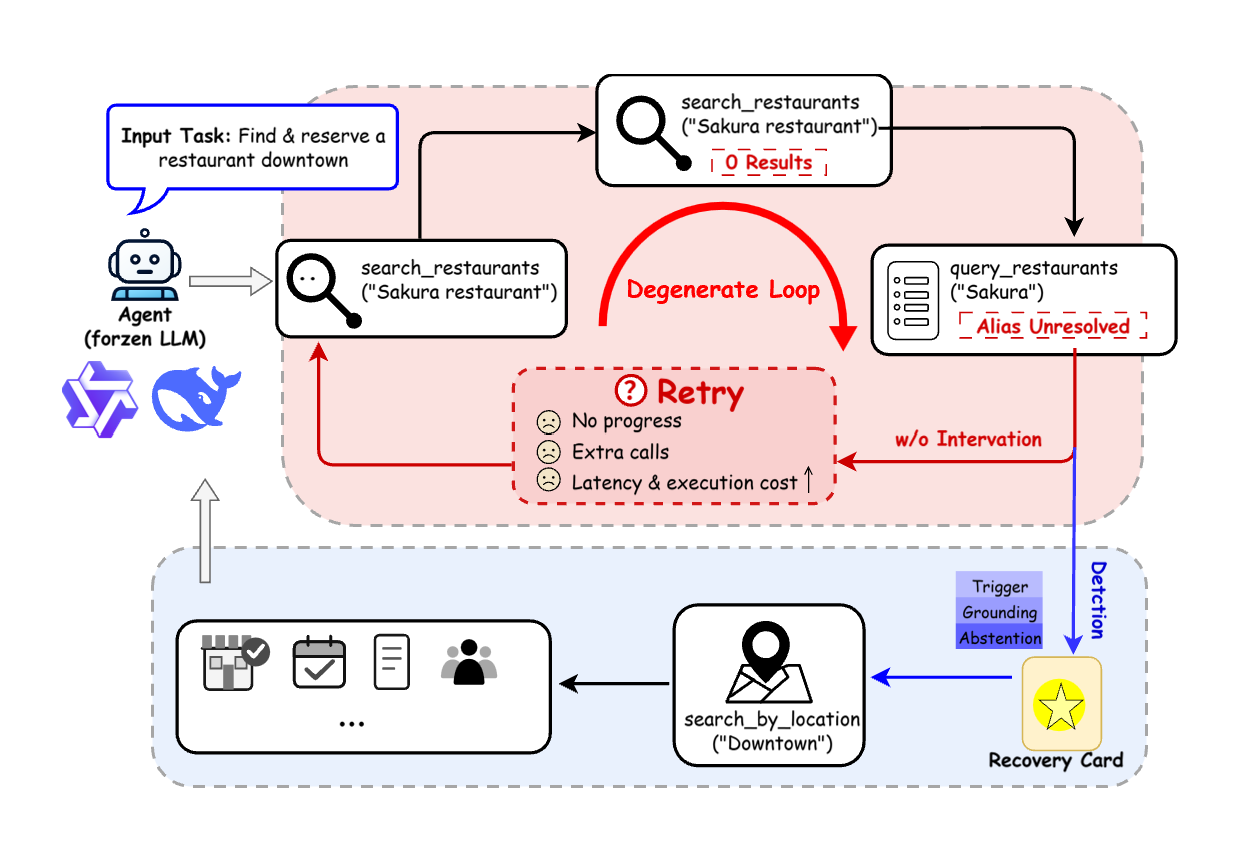
\includegraphics[width=\columnwidth]{figures/fig_persist_ace_escape_overview.png}
    \caption{Illustrative Functional Loop and local escape. After earlier feedback is
    visible, different search and query calls repeat the same unresolved effect
    without progress. PERSIST-ACE admits a grounded location-search Card, makes
    one bounded correction, and returns control to the base LLM.}
    \label{fig:escape-example}
\end{figure}

Existing defenses leave a gap. Exact-repeat blockers miss surface-diverse
failures, early stopping abandons states that may still be recoverable, and
online replanning adds another generation step without guaranteeing a grounded
action. Detection alone is also insufficient: a retry may still be productive,
and some stalled states have no unique safe repair.

We present \textbf{PERSIST-ACE}, which learns bounded recovery programs from
earlier failures. Figure~\ref{fig:framework} shows the full path. Offline, it
compiles recurring effect-level failure patterns into typed Recovery Cards
with explicit triggers, grounding rules, abstention conditions, and budgets.
Online, no-progress recalls a candidate, repeated effect confirms a Functional Loop, and
the controller either admits one grounded Card or preserves the Raw action.
Control then returns to the base LLM without updating its policy or invoking
open-ended replanning.

We evaluate PERSIST-ACE on STATE-Bench, DeepPlanning Shopping, and
$\tau$-Knowledge. The method improves the primary task outcome on all three
benchmarks, and the mechanism study attributes the strongest recovery behavior
to selective, grounded Cards rather than detection or generic prompting alone.

Our contributions are threefold:
\begin{itemize}
    \item \textbf{Functional Loop analysis.} We formalize a Functional Loop as no progress
    plus a feedback-visible repeated functional effect, characterize how it
    varies by model and benchmark, and show why tool-name repetition
    is an inadequate proxy.
    \item \textbf{Programmatic action recovery.} We introduce PERSIST-ACE, an
    offline experience compiler and online selective controller for grounded,
    bounded recovery programs.
    \item \textbf{Evaluation.} We show improved primary task outcomes on three
    tool-use benchmarks and use controlled ablations to separate Card
    validation, grounding, and recovery-program effects.
\end{itemize}
